
% ---- closed --------

\begin{figure}[!htb]
    \centering
    \begin{minipage}[b]{0.45\textwidth}
        \centering
        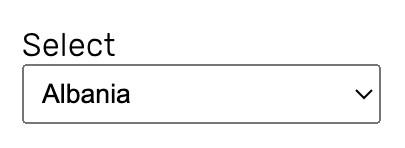
\includegraphics[width=0.8\textwidth]{closed.osx.chrome.png}
        \caption{Geschlossene Datalist auf OSX Chrome}
        \label{img:closedOsxChromeDatalist}
    \end{minipage}
    \hfill
    \begin{minipage}[b]{0.45\textwidth}
        \centering
        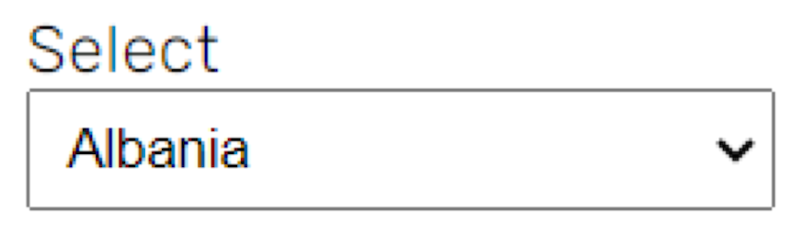
\includegraphics[width=0.8\textwidth]{closed.win.chrome.png}
        \caption{Geschlossene Datalist auf Windows Chrome}
        \label{img:closedWinChromeDatalist}
    \end{minipage}
\end{figure}

\begin{figure}[!htb]
    \centering
    \begin{minipage}[b]{0.45\textwidth}
        \centering
        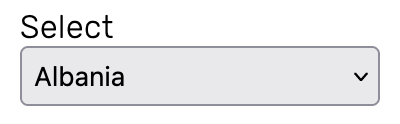
\includegraphics[width=0.8\textwidth]{closed.osx.firefox.png}
        \caption{Geschlossene Datalist auf OSX Firefox}
        \label{img:closedOsxFirefoxDatalist}
    \end{minipage}
    \hfill
    \begin{minipage}[b]{0.45\textwidth}
        \centering
        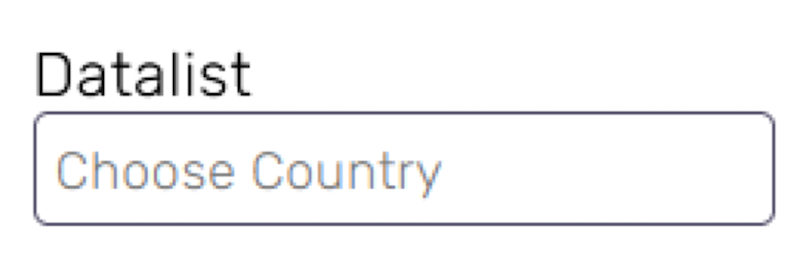
\includegraphics[width=0.8\textwidth]{closed.win.firefox.png}
        \caption{Geschlossene Datalist auf Windows Firefox}
        \label{img:closedWinFirefoxDatalist}
    \end{minipage}
\end{figure}

\begin{figure}[!htb]
    \centering
    \begin{minipage}[b]{0.45\textwidth}
        \centering
        
\includegraphics[width=0.8\textwidth]{closed.osx.safari.png}
        \caption{Geschlossene Datalist auf OSX Safari}
        \label{img:closedOsxSafariDatalist}
    \end{minipage}
    \hfill
    \begin{minipage}[b]{0.45\textwidth}
        \centering
        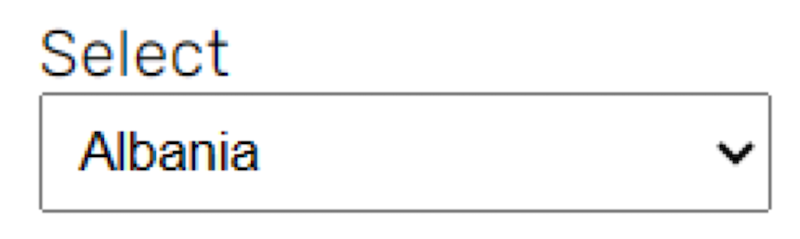
\includegraphics[width=0.8\textwidth]{closed.win.edge.png}
        \caption{Geschlossene Datalist auf Windows Edge}
        \label{img:closedWinEdgeDatalist}
    \end{minipage}
\end{figure}

% ---- opened --------

\begin{figure}[!htb]
    \centering
    \begin{minipage}[b]{0.45\textwidth}
        \centering
        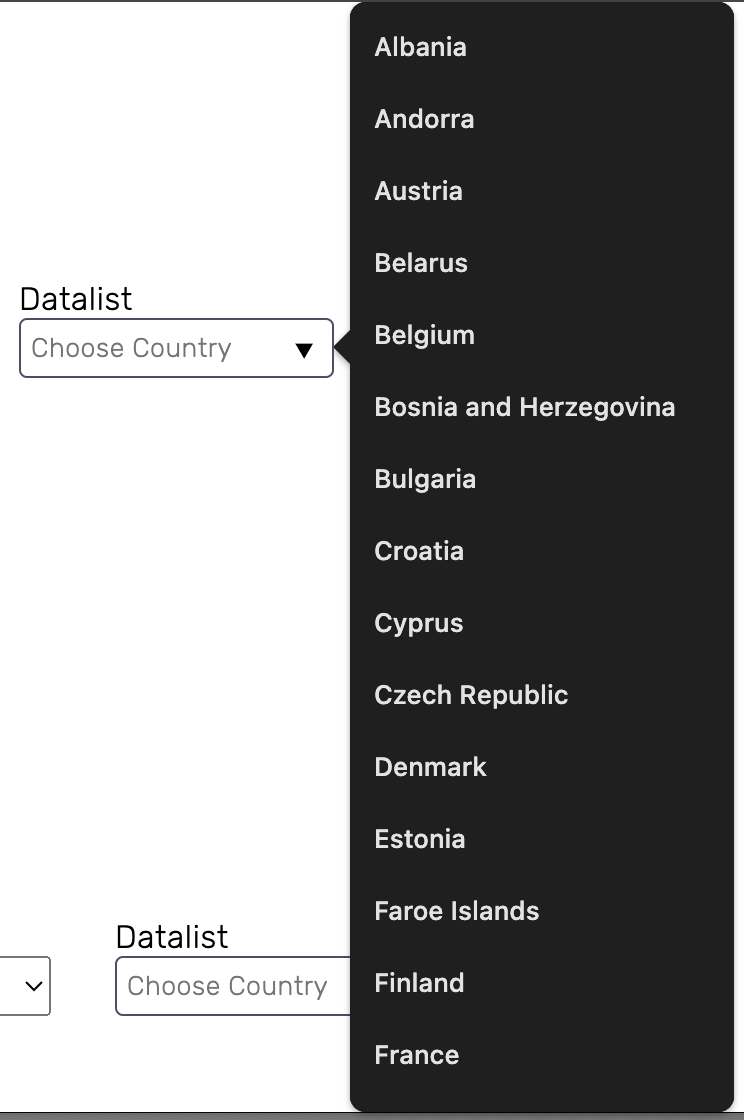
\includegraphics[width=0.65\textwidth]{opened.osx.chrome.png}
        \caption{Offene Datalist auf OSX Chrome}
        \label{img:openedOsxChromeDatalist}
    \end{minipage}
    \hfill
    \begin{minipage}[b]{0.45\textwidth}
        \centering
        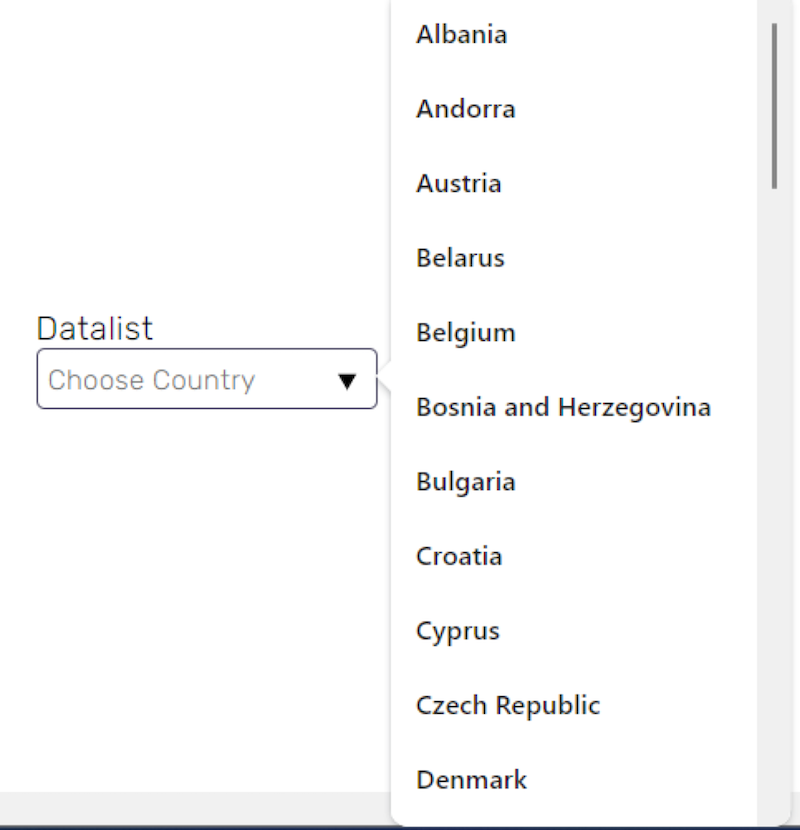
\includegraphics[width=0.85\textwidth]{opened.win.chrome.png}
        \caption{Offene Datalist auf Windows Chrome}
        \label{img:openedWinChromeDatalist}
    \end{minipage}
\end{figure}

\begin{figure}[!htb]
    \centering
    \begin{minipage}[b]{0.45\textwidth}
        \centering
        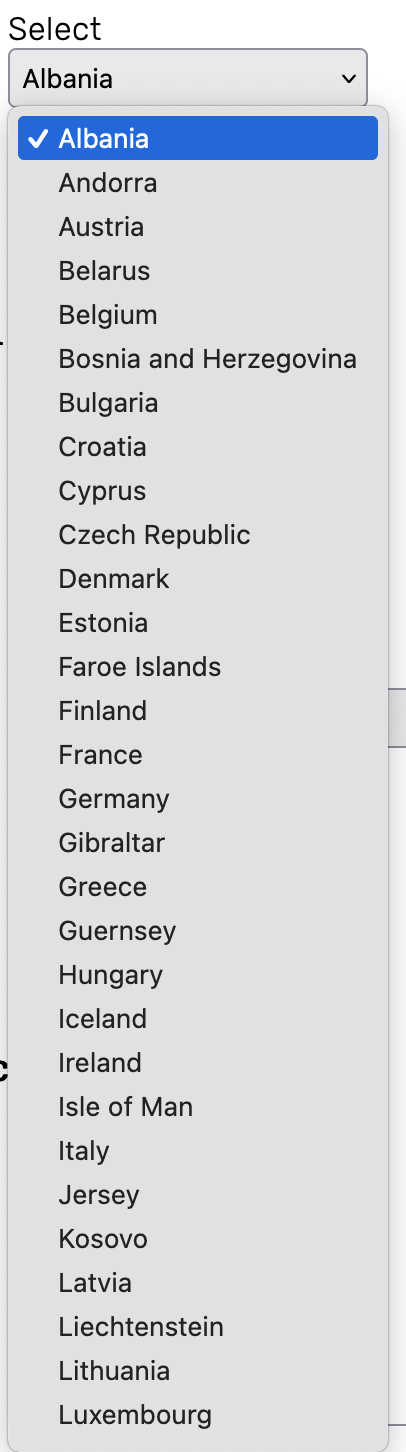
\includegraphics[width=0.6\textwidth]{opened.osx.firefox.png}
        \caption{Offene Datalist auf OSX Firefox}
        \label{img:openedOsxFirefoxDatalist}
    \end{minipage}
    \hfill
    \begin{minipage}[b]{0.45\textwidth}
        \centering
        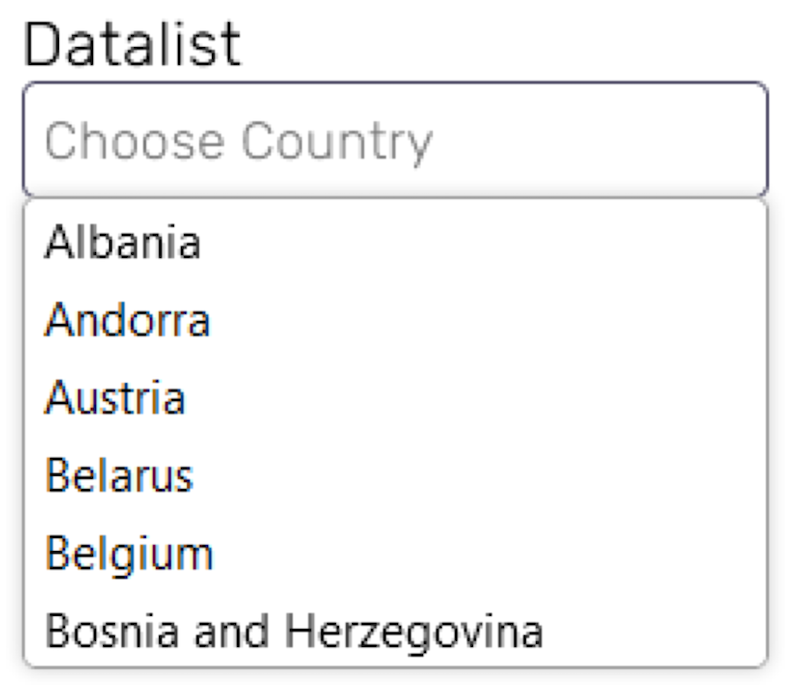
\includegraphics[width=0.6\textwidth]{opened.win.firefox.png}
        \caption{Offene Datalist auf Windows Firefox}
        \label{img:openedWinFirefoxDatalist}
    \end{minipage}
\end{figure}

\begin{figure}[!htb]
    \centering
    \begin{minipage}[b]{0.5\textwidth}
        \centering
        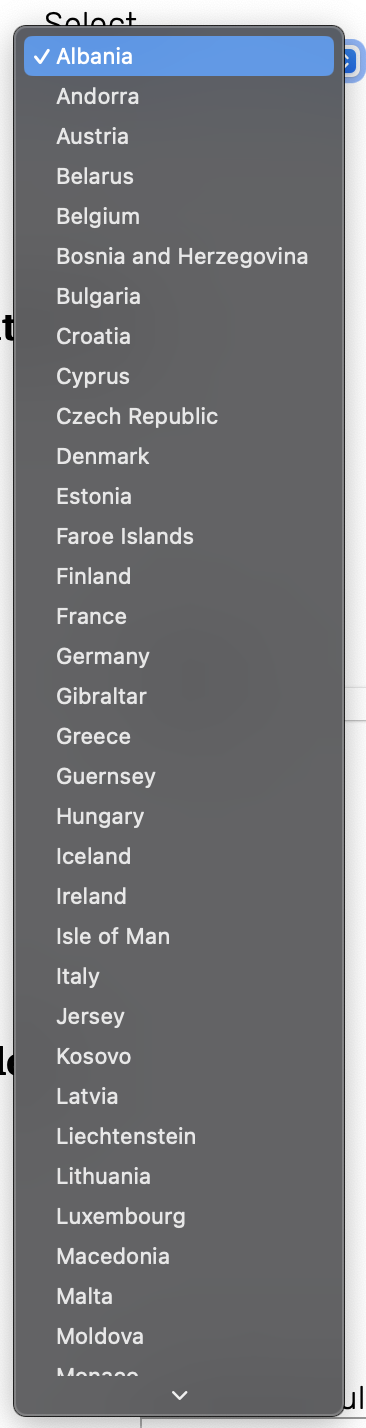
\includegraphics[width=0.6\textwidth]{opened.osx.safari.png}
        \caption{Offene Datalist auf OSX Safari}
        \label{img:openedOsxSafariDatalist}
    \end{minipage}
    \hfill
    \begin{minipage}[b]{0.45\textwidth}
        \centering
        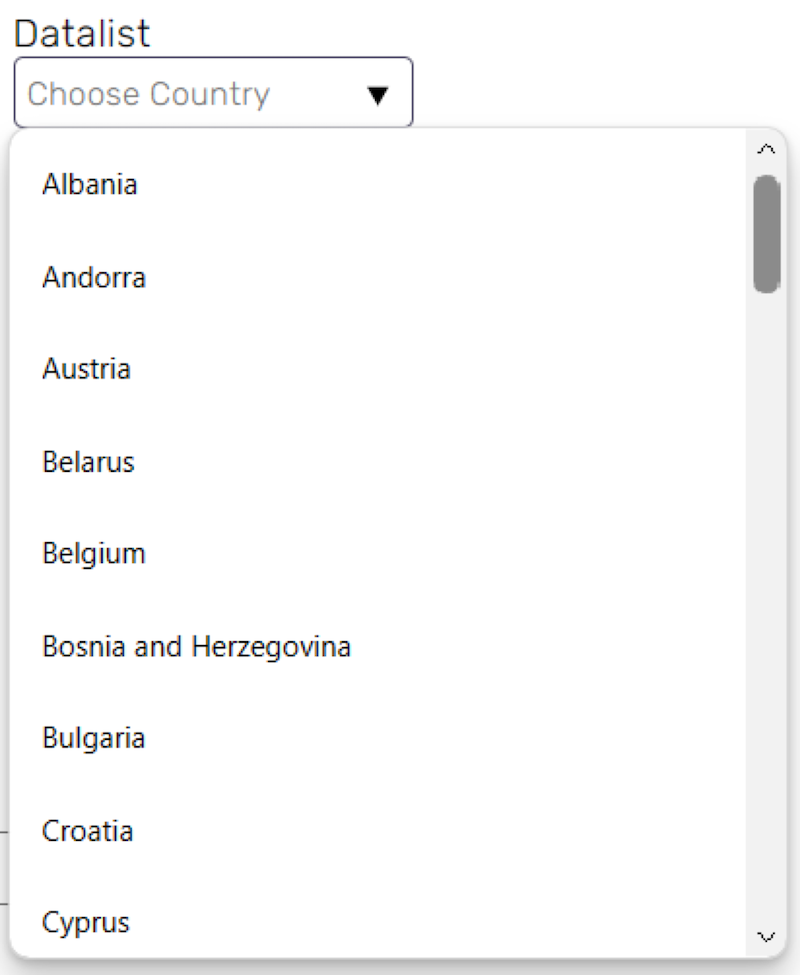
\includegraphics[width=0.6\textwidth]{opened.win.edge.png}
        \caption{Offene Datalist auf Windows Edge}
        \label{img:openedWinEdgeDatalist}
    \end{minipage}
\end{figure}

% ---- mobile --------

\begin{figure}[!htb]
    \centering
    \begin{minipage}[b]{0.45\textwidth}
        \centering
        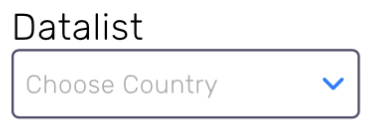
\includegraphics[width=0.8\textwidth]{closed.ios.safari.png}
        \caption{Geschlossene Datalist auf iOS Safari}
        \label{img:closedIosSafariDatalist}
    \end{minipage}
    \hfill
    \begin{minipage}[b]{0.45\textwidth}
        \centering
        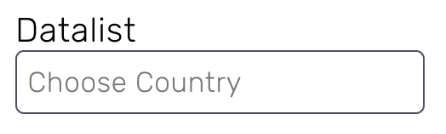
\includegraphics[width=0.8\textwidth]{closed.android.firefox.png}
        \caption{Geschlossene Datalist auf Android Firefox}
        \label{img:closedAndroidFirefoxDatalist}
    \end{minipage}
\end{figure}

\begin{figure}[!htb]
    \centering
    \begin{minipage}[b]{0.45\textwidth}
        \centering
        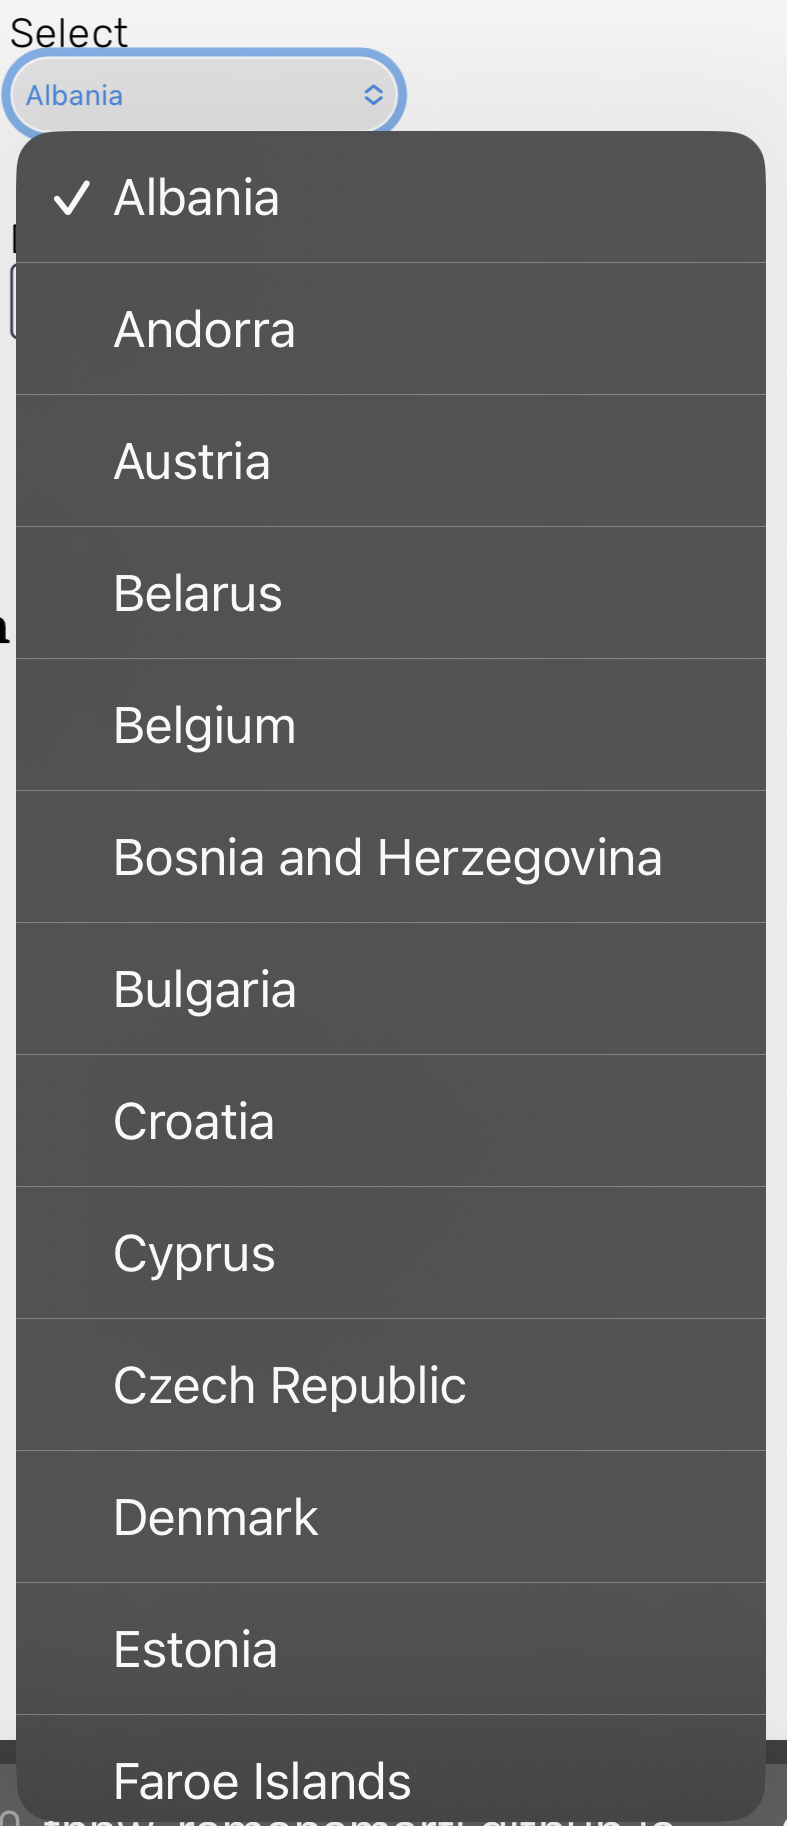
\includegraphics[width=0.6\textwidth]{opened.ios.safari.png}
        \caption{Offene Datalist auf iOS Safari}
        \label{img:openedIosSafariDatalist}
    \end{minipage}
    \hfill
    \begin{minipage}[b]{0.45\textwidth}
        \centering
        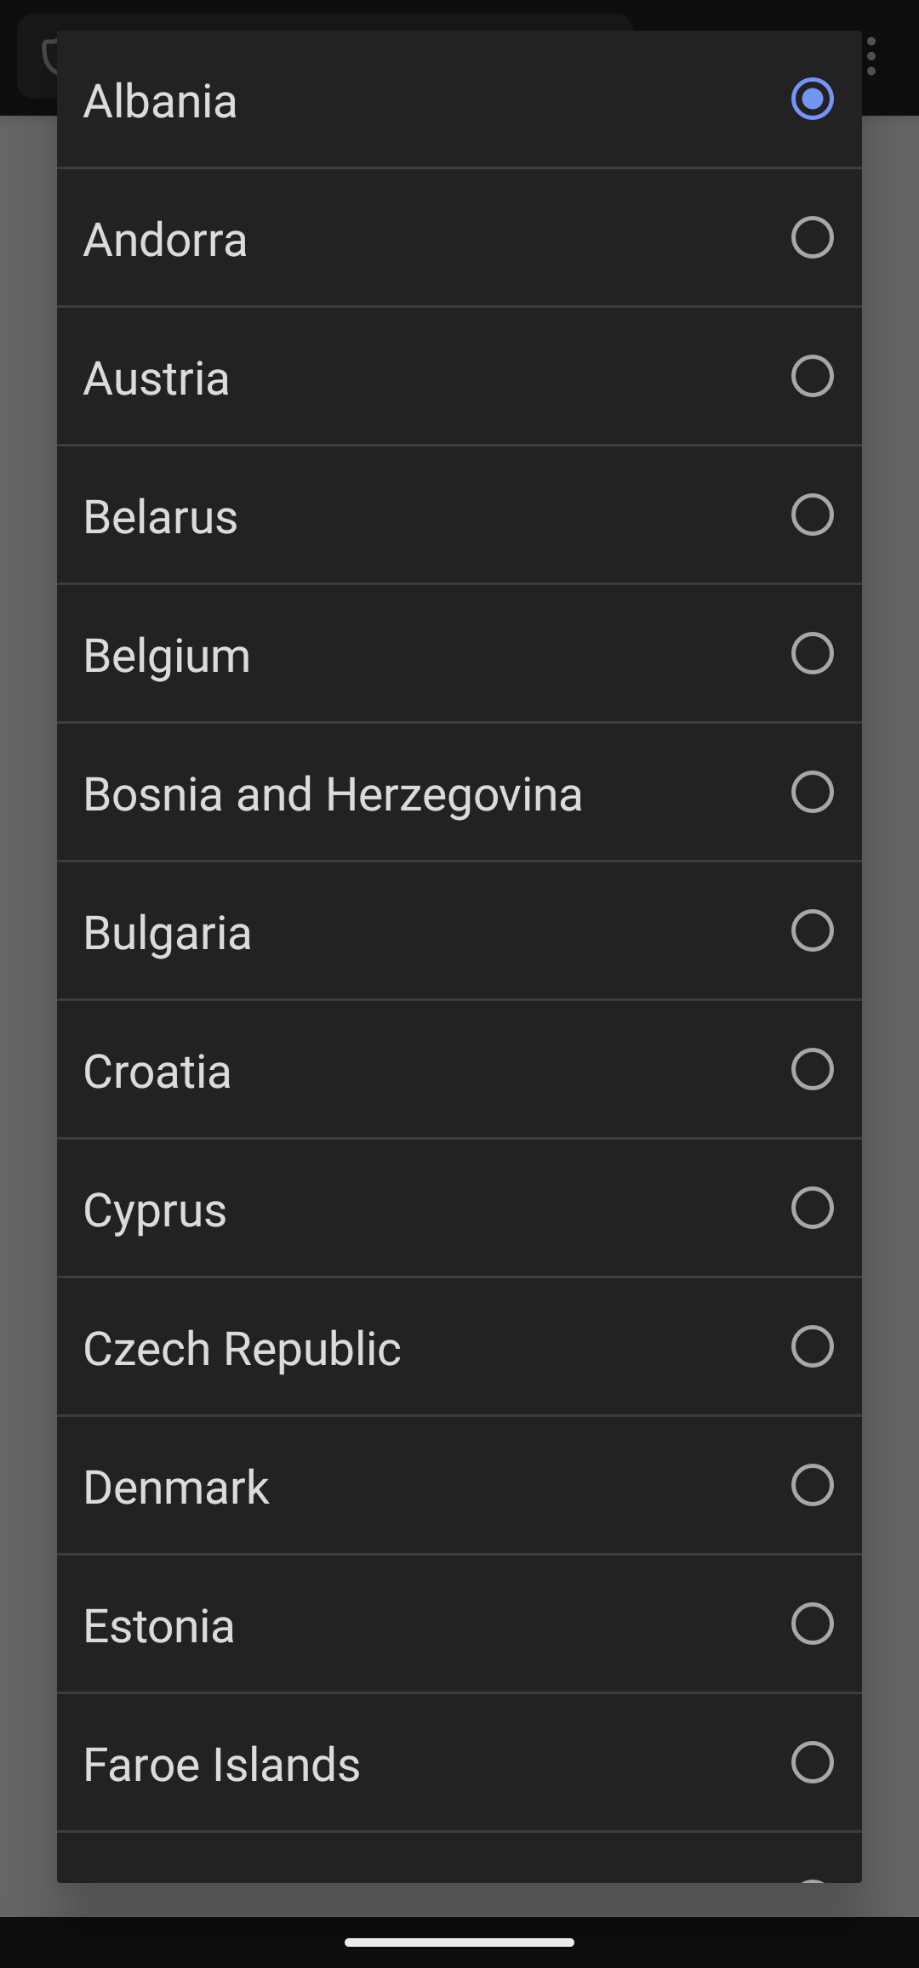
\includegraphics[width=0.45\textwidth]{opened.android.duckduck.png}
        \caption{Offene Datalist auf Android DuckduckGo}
        \label{img:openedAndroidDuckduckDatalist}
    \end{minipage}
\end{figure}

% ---- disabled --------

\begin{figure}[!htb]
    \centering
    \begin{minipage}[b]{0.45\textwidth}
        \centering
        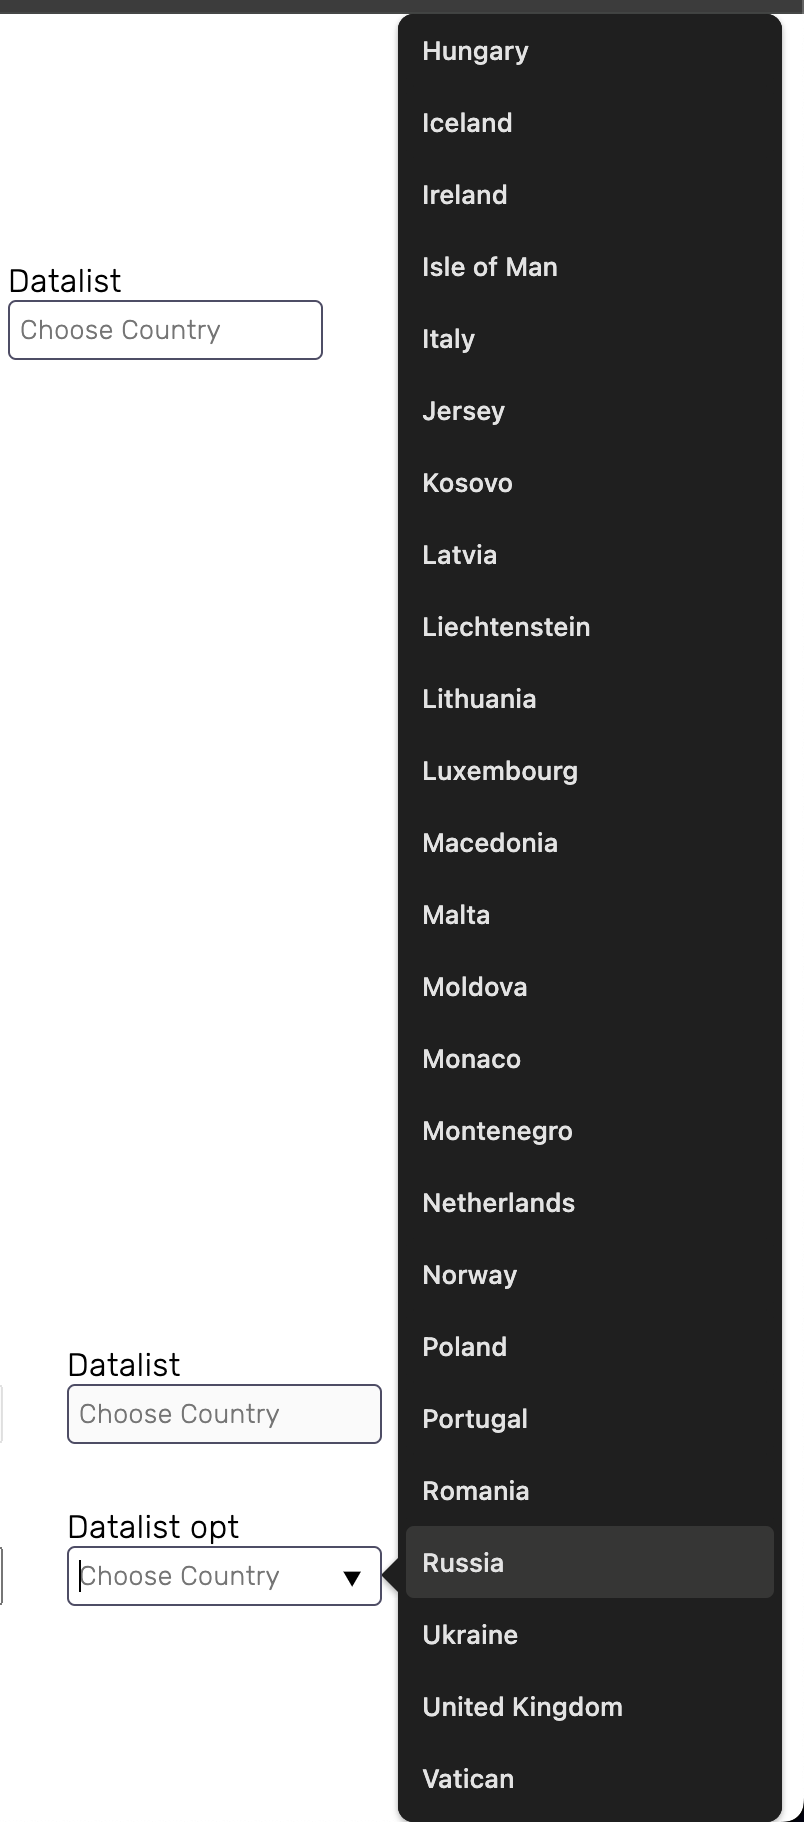
\includegraphics[width=0.8\textwidth]{disabled.osx.chrome.png}
        \caption{Disabled Datalist auf OSX Chrome}
        \label{img:disabledOsxChromeDatalist}
    \end{minipage}
    \hfill
    \begin{minipage}[b]{0.45\textwidth}
        \centering
        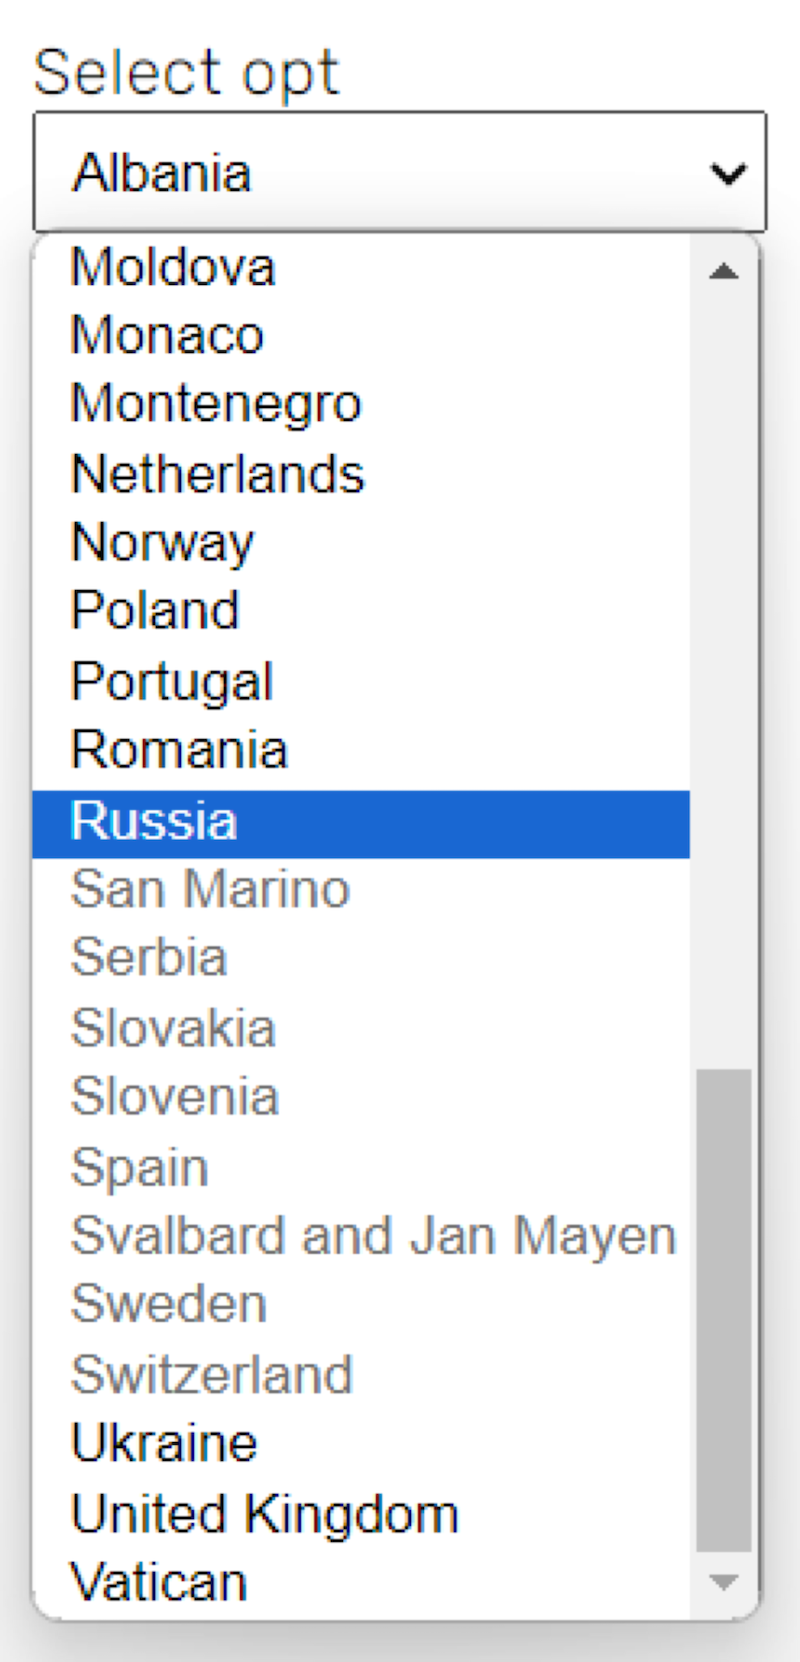
\includegraphics[width=0.8\textwidth]{disabled.win.chrome.png}
        \caption{Disabled Datalist auf Windows Chrome}
        \label{img:disabledWinChromeDatalist}
    \end{minipage}
\end{figure}

\begin{figure}[!htb]
    \centering
    \begin{minipage}[b]{0.45\textwidth}
        \centering
        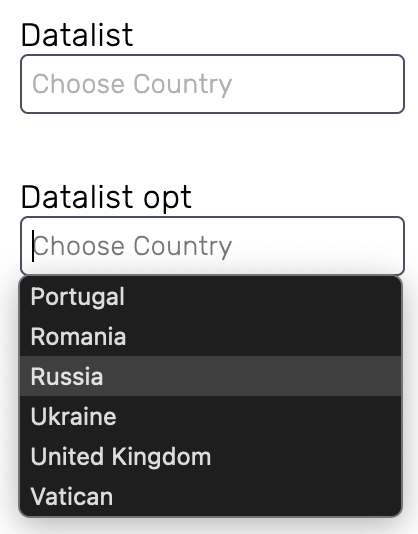
\includegraphics[width=0.8\textwidth]{disabled.osx.firefox.png}
        \caption{Disabled Datalist auf OSX Firefox}
        \label{img:disabledOsxFirefoxDatalist}
    \end{minipage}
    \hfill
    \begin{minipage}[b]{0.45\textwidth}
        \centering
        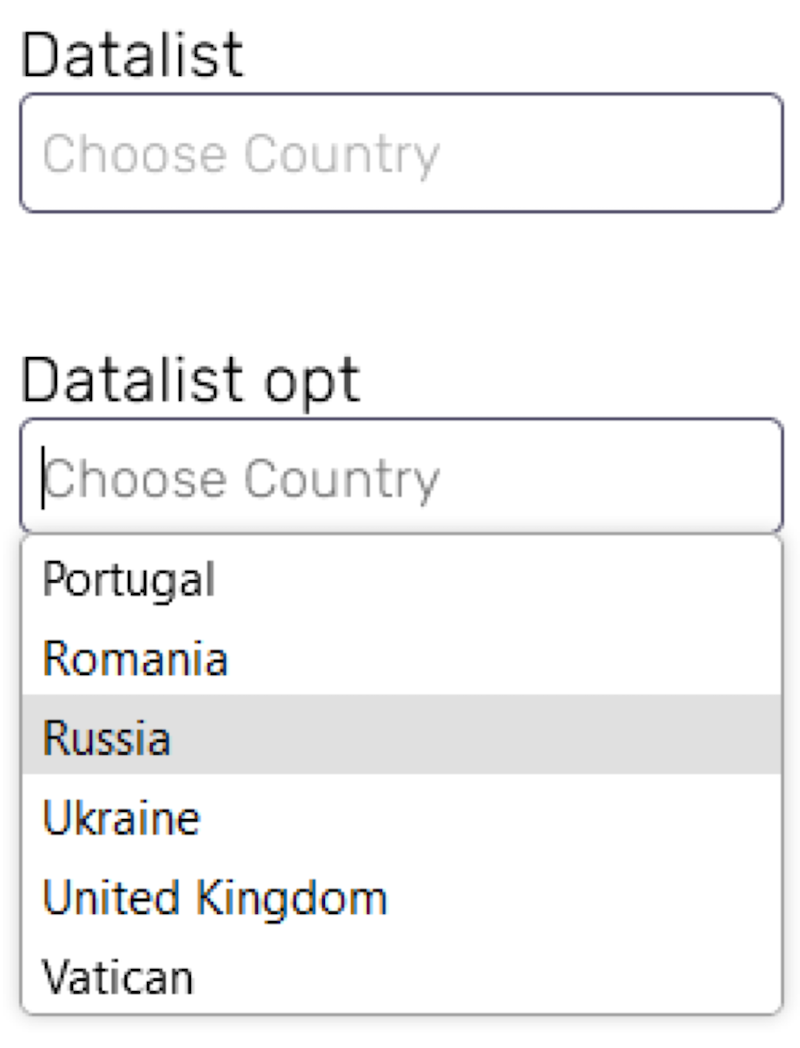
\includegraphics[width=0.8\textwidth]{disabled.win.firefox.png}
        \caption{Disabled Datalist auf Windows Firefox}
        \label{img:disabledWinFirefoxDatalist}
    \end{minipage}
\end{figure}

\begin{figure}[!htb]
    \centering
    \begin{minipage}[b]{0.45\textwidth}
        \centering
        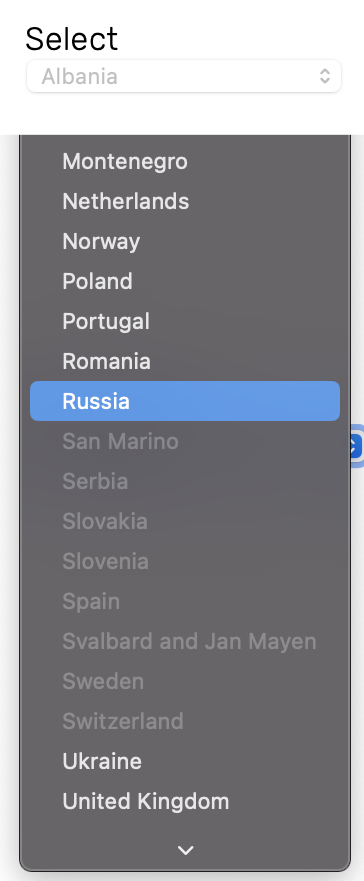
\includegraphics[width=0.8\textwidth]{disabled.osx.safari.png}
        \caption{Disabled Datalist auf OSX Safari}
        \label{img:disabledOsxSafariDatalist}
    \end{minipage}
    \hfill
    \begin{minipage}[b]{0.45\textwidth}
        \centering
        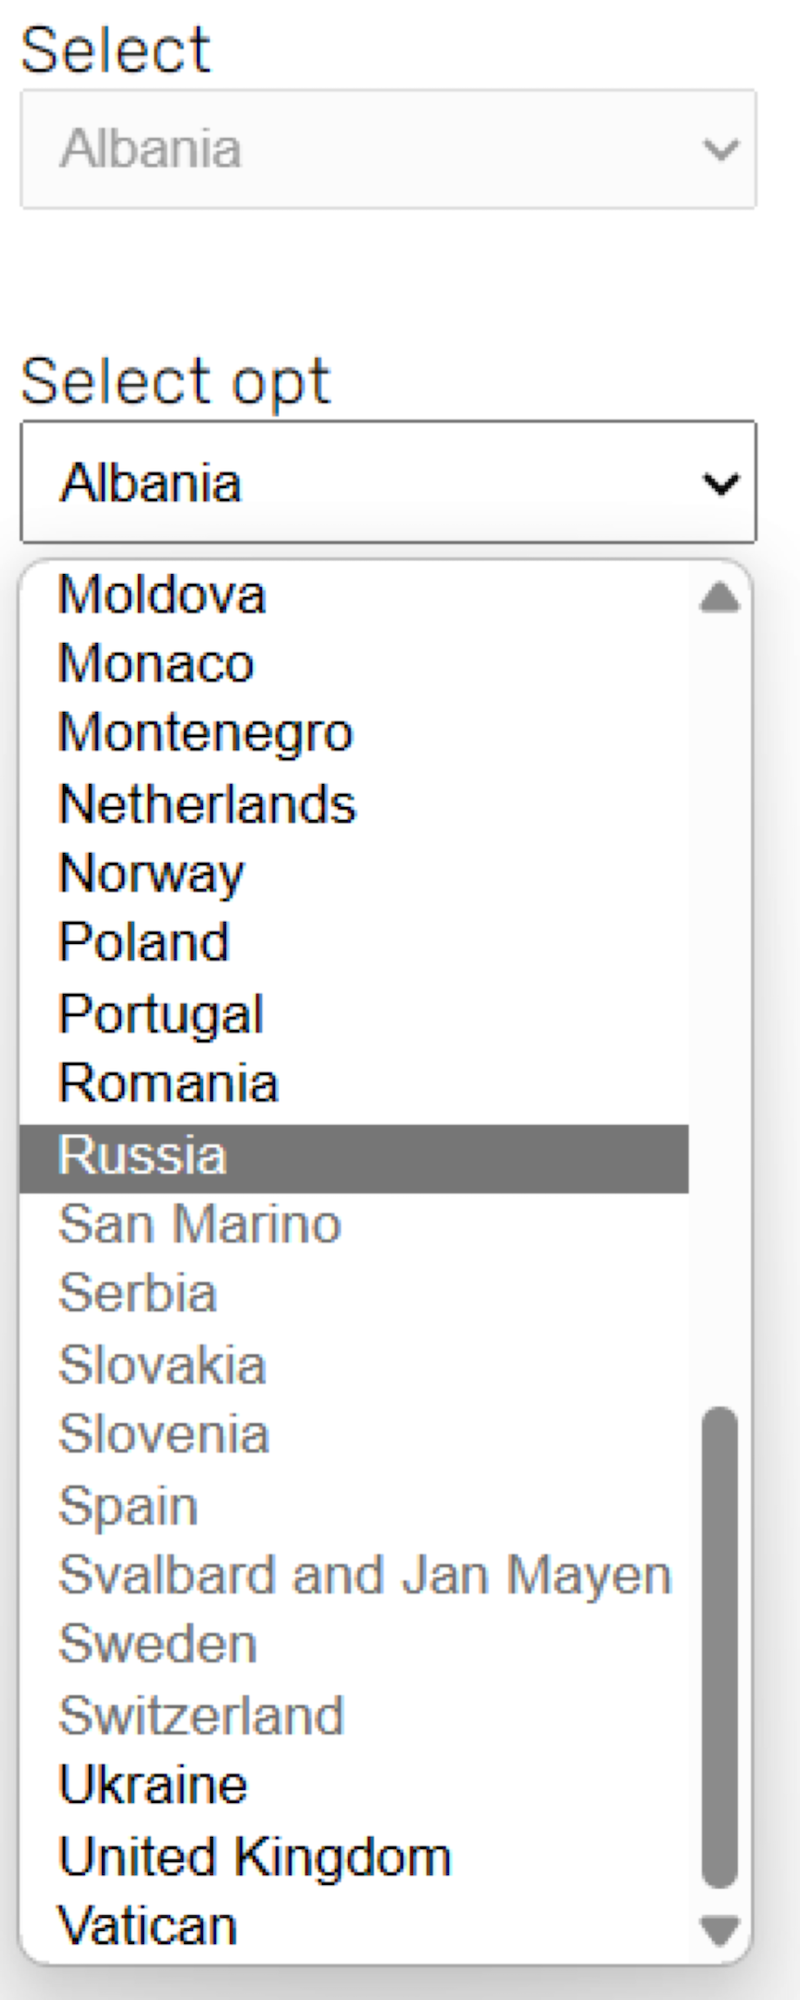
\includegraphics[width=0.8\textwidth]{disabled.win.edge.png}
        \caption{Disabled Datalist auf Windows Edge}
        \label{img:disabledWinEdgeDatalist}
    \end{minipage}
\end{figure}

% ---- labeled --------

\begin{figure}[!htb]
    \centering
    \begin{minipage}[b]{0.45\textwidth}
        \centering
        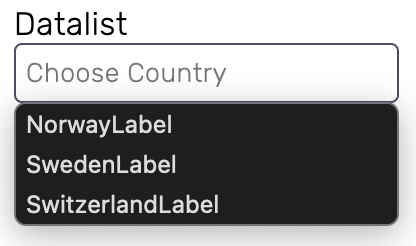
\includegraphics[width=0.6\textwidth]{labeled.osx.firefox.png}
        \caption{Labeled Datalist auf OSX Firefox}
        \label{img:labeledOsxFirefoxDatalist}
    \end{minipage}
    \hfill
    \begin{minipage}[b]{0.45\textwidth}
        \centering
        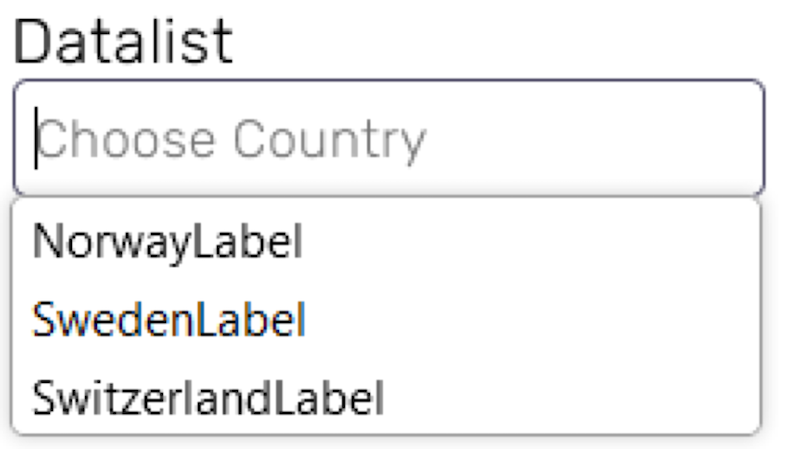
\includegraphics[width=0.6\textwidth]{labeled.win.firefox.png}
        \caption{Labeled Datalist auf Windows Firefox}
        \label{img:labeledWinFirefoxDatalist}
    \end{minipage}
\end{figure}

\begin{figure}[!htb]
    \centering
    \begin{minipage}[b]{0.45\textwidth}
        \centering
        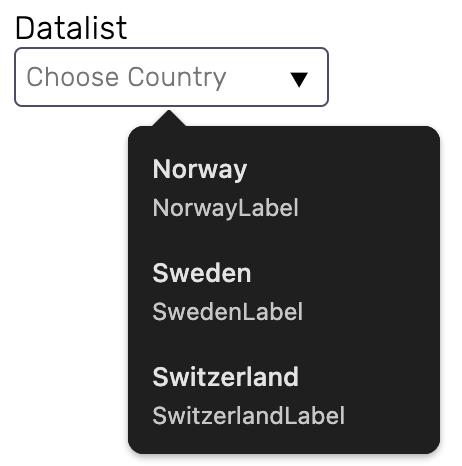
\includegraphics[width=0.8\textwidth]{labeled.osx.chrome.png}
        \caption{Labeled Datalist auf OSX Chrome}
        \label{img:labeledOsxChromeDatalist}
    \end{minipage}
    \hfill
    \begin{minipage}[b]{0.45\textwidth}
        \centering
        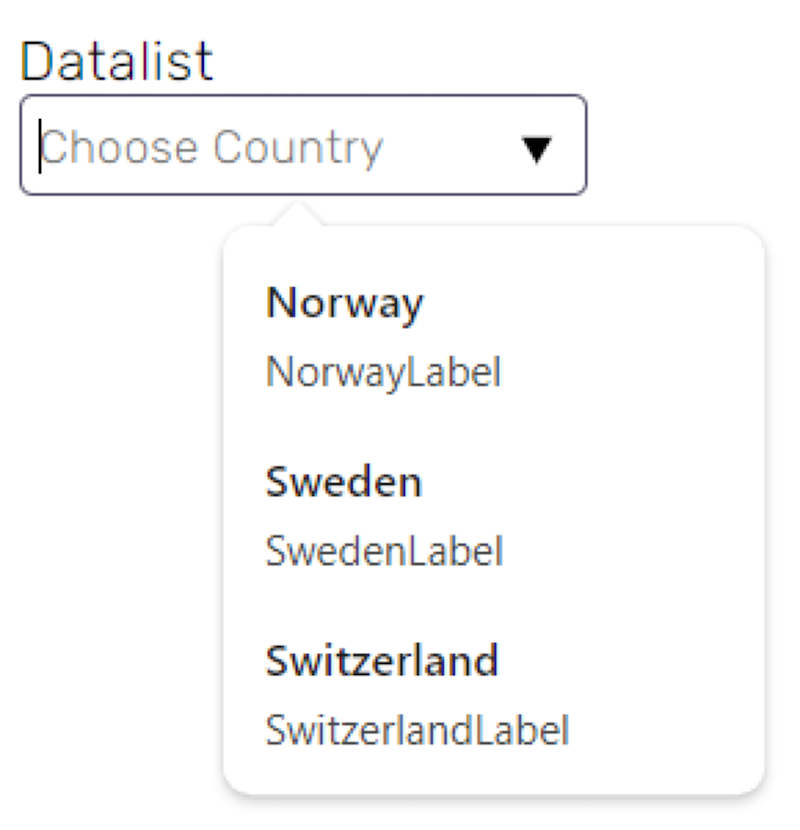
\includegraphics[width=0.8\textwidth]{labeled.win.chrome.png}
        \caption{Labeled Datalist auf Windows Chrome}
        \label{img:labeledWinChromeDatalist}
    \end{minipage}
\end{figure}

\begin{figure}[!htb]
    \centering
    \begin{minipage}[b]{0.45\textwidth}
        \centering
        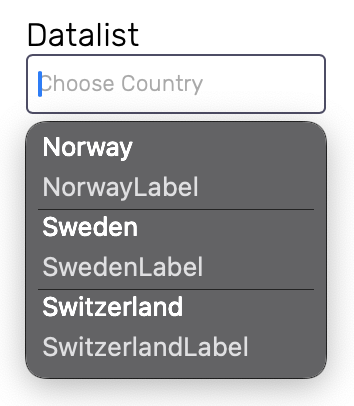
\includegraphics[width=0.6\textwidth]{labeled.osx.safari.png}
        \caption{Labeled Datalist auf OSX Safari}
        \label{img:labeledOsxSafariDatalist}
    \end{minipage}
    \hfill
    \begin{minipage}[b]{0.45\textwidth}
        \centering
        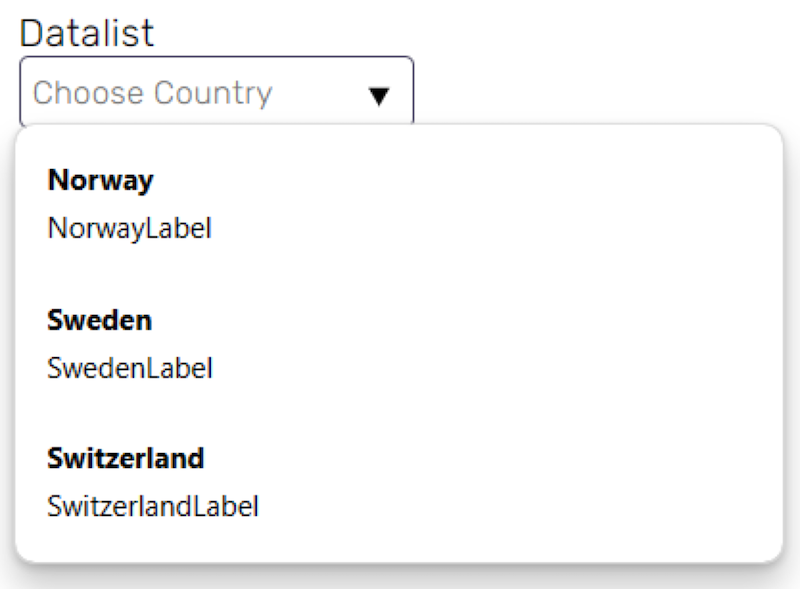
\includegraphics[width=0.8\textwidth]{labeled.win.edge.png}
        \caption{Labeled Datalist auf Windows Edge}
        \label{img:labeledWinEdgeDatalist}
    \end{minipage}
\end{figure}

% ---- specials - range --------

\begin{figure}[!htb]
    \centering
    \begin{minipage}[b]{0.28\textwidth}
        \centering
        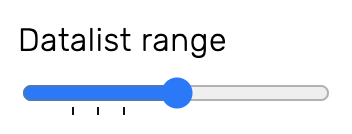
\includegraphics[width=0.9\textwidth]{range.osx.chrome.png}
        \caption{Range-Datalist auf OSX Chrome}
        \label{img:rangeOsxChromeDatalist}
    \end{minipage}
    \hfill
    \begin{minipage}[b]{0.28\textwidth}
        \centering
        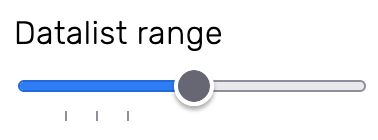
\includegraphics[width=0.9\textwidth]{range.osx.firefox.png}
        \caption{Range-Datalist auf OSX Firefox}
        \label{img:rangeOsxFirefoxDatalist}
    \end{minipage}
    \hfill
    \begin{minipage}[b]{0.28\textwidth}
        \centering
        
\includegraphics[width=0.9\textwidth]{range.osx.safari.png}
        \caption{Range-Datalist auf OSX Safari}
        \label{img:rangeOsxSafariDatalist}
    \end{minipage}
\end{figure}

\begin{figure}[!htb]
    \centering
    \begin{minipage}[b]{0.28\textwidth}
        \centering
        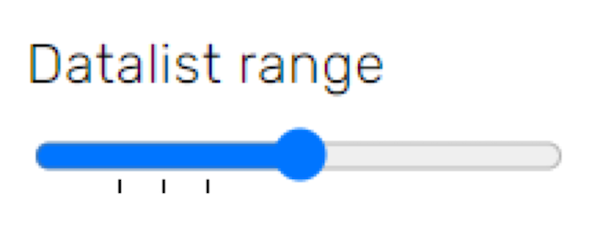
\includegraphics[width=0.9\textwidth]{range.win.chrome.png}
        \caption{Range-Datalist auf Windows Chrome}
        \label{img:rangeWinChromeDatalist}
    \end{minipage}
    \hfill
    \begin{minipage}[b]{0.28\textwidth}
        \centering
        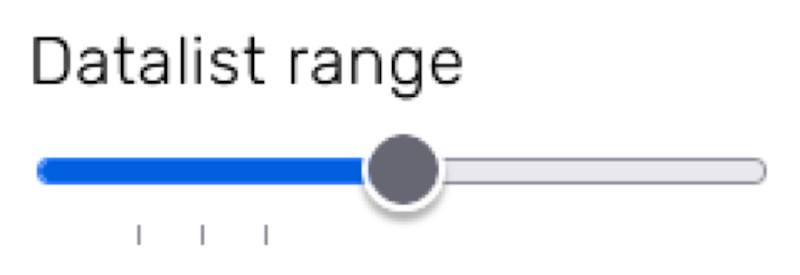
\includegraphics[width=0.9\textwidth]{range.win.firefox.png}
        \caption{Range-Datalist auf Windows Firefox}
        \label{img:rangeWinFirefoxDatalist}
    \end{minipage}
    \hfill
    \begin{minipage}[b]{0.28\textwidth}
        \centering
        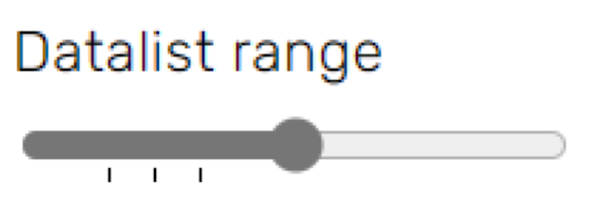
\includegraphics[width=0.9\textwidth]{range.win.edge.png}
        \caption{Range-Datalist auf Windows Edge}
        \label{img:rangeWinEdgeDatalist}
    \end{minipage}
\end{figure}

% ---- specials - color --------

\begin{figure}[!htb]
    \centering
    \begin{minipage}[b]{0.28\textwidth}
        \centering
        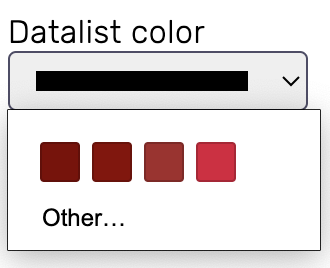
\includegraphics[width=0.9\textwidth]{color.osx.chrome.png}
        \caption{Color-Datalist auf OSX Chrome}
        \label{img:colorOsxChromeDatalist}
    \end{minipage}
    \hfill
    \begin{minipage}[b]{0.28\textwidth}
        \centering
        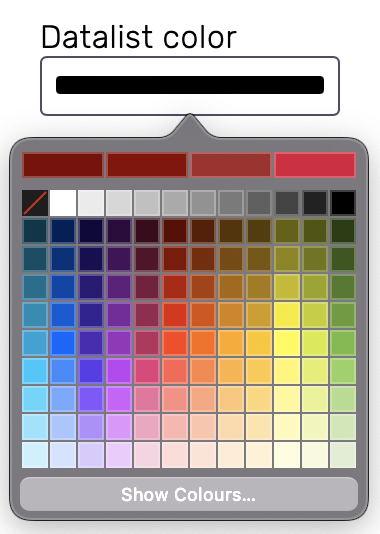
\includegraphics[width=0.8\textwidth]{color.osx.safari.png}
        \caption{Color-Datalist auf OSX Safari}
        \label{img:colorOsxSafariDatalist}
    \end{minipage}
    \hfill
    \begin{minipage}[b]{0.28\textwidth}
        \centering
        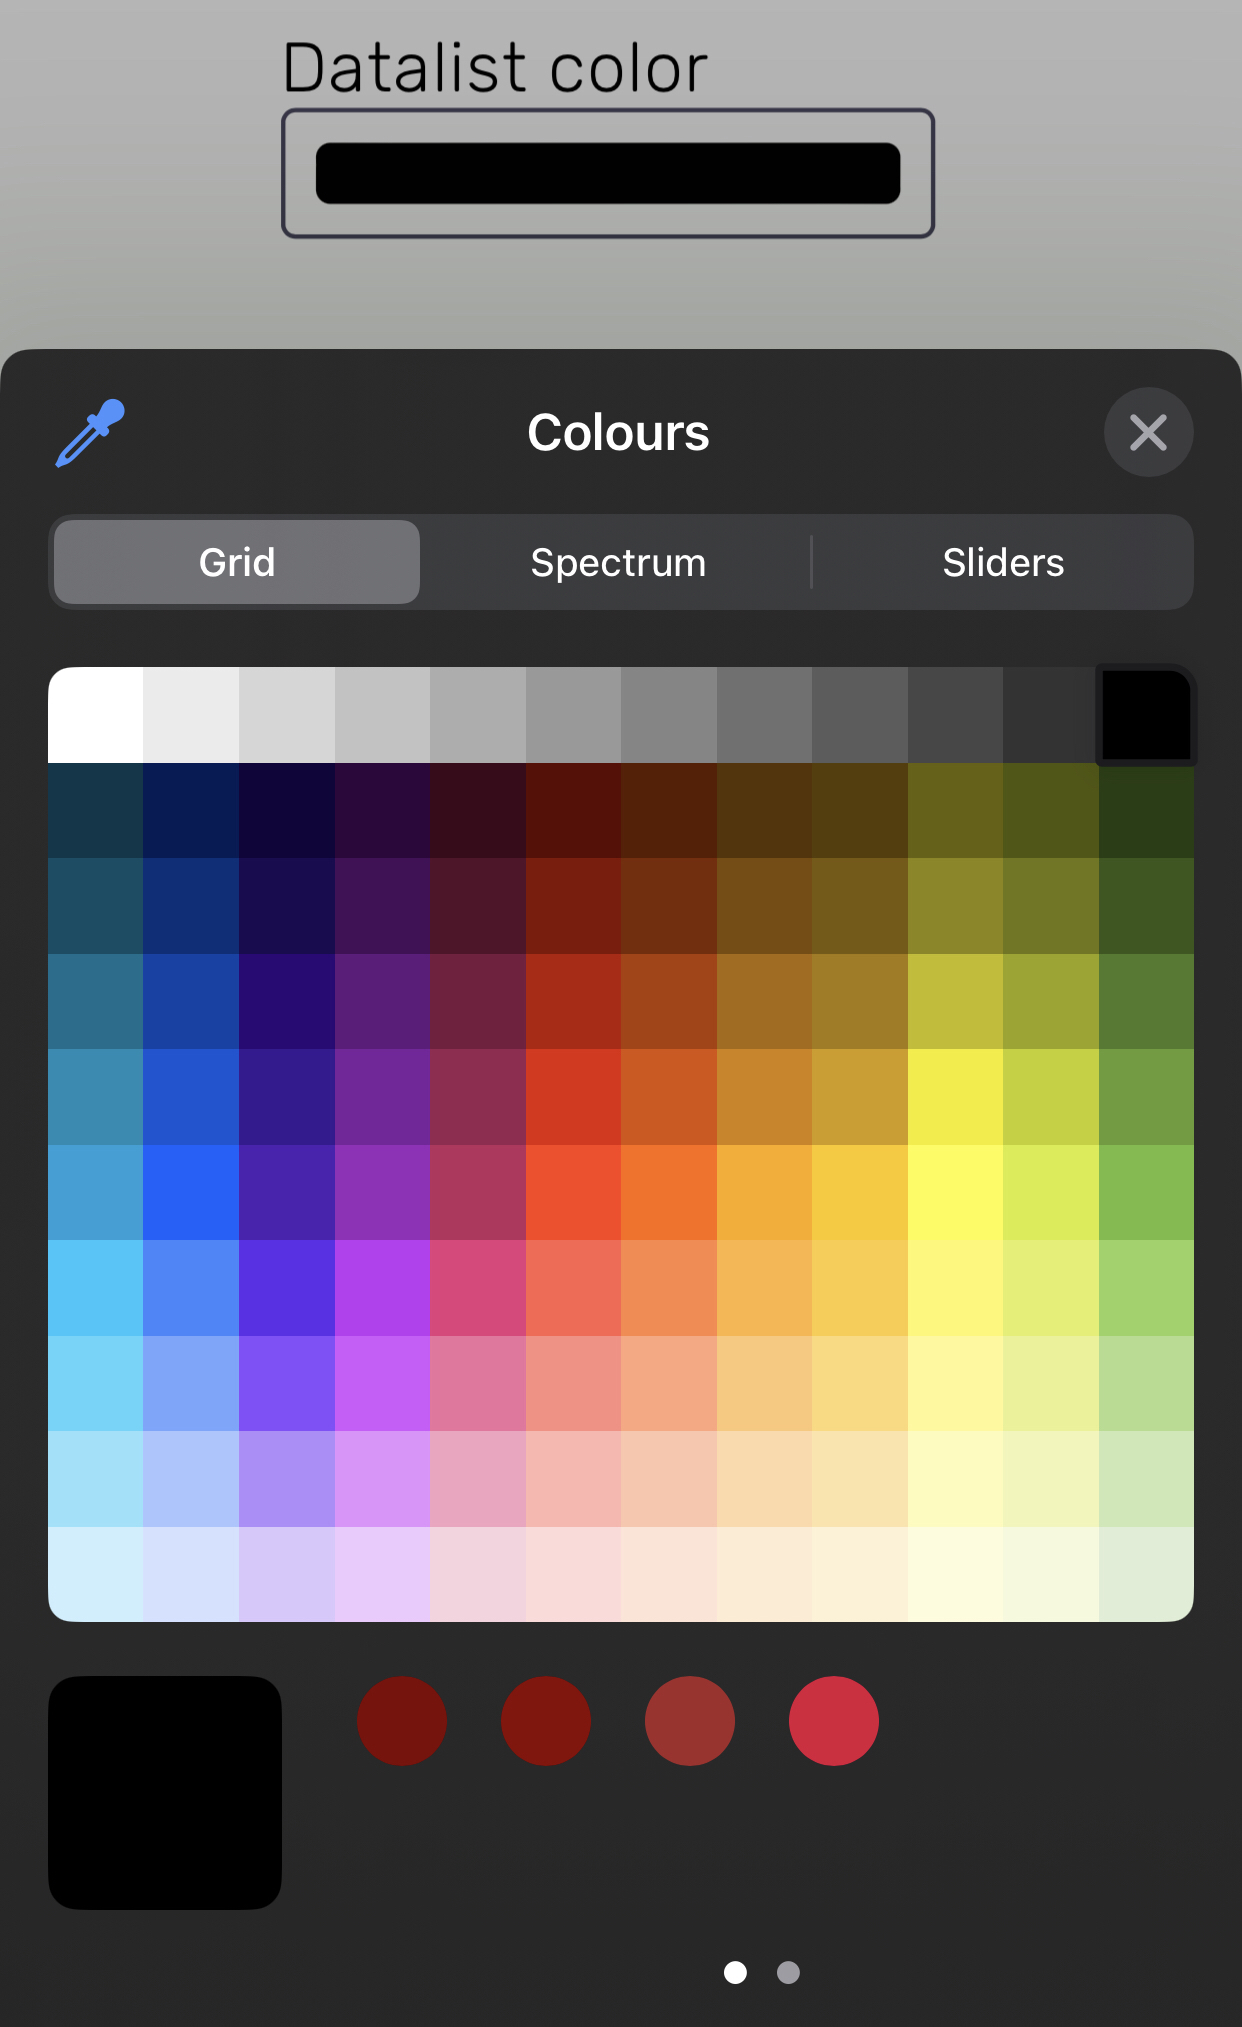
\includegraphics[width=0.6\textwidth]{color.ios.safari.png}
        \caption{Color-Datalist auf iOS Safari}
        \label{img:colorIsoSafariDatalist}
    \end{minipage}
\end{figure}

\begin{figure}[!htb]
    \centering
    \begin{minipage}[b]{0.28\textwidth}
        \centering
        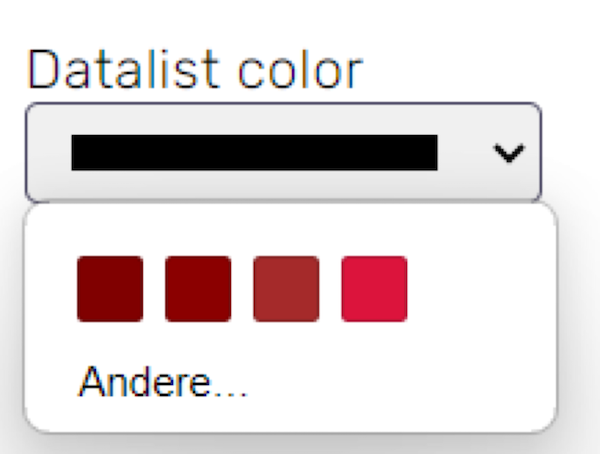
\includegraphics[width=0.9\textwidth]{color.win.chrome.png}
        \caption{Color-Datalist auf Windows Chrome}
        \label{img:colorWinChromeDatalist}
    \end{minipage}
    \hfill
    \begin{minipage}[b]{0.28\textwidth}
        \centering
        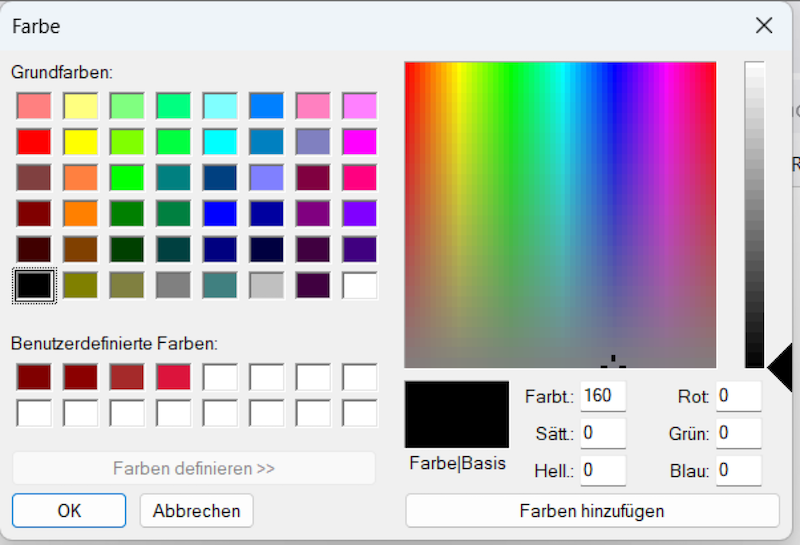
\includegraphics[width=0.9\textwidth]{color.win.firefox.png}
        \caption{Color-Datalist auf Windows Firefox}
        \label{img:colorWinFirefoxDatalist}
    \end{minipage}
    \hfill
    \begin{minipage}[b]{0.28\textwidth}
        \centering
        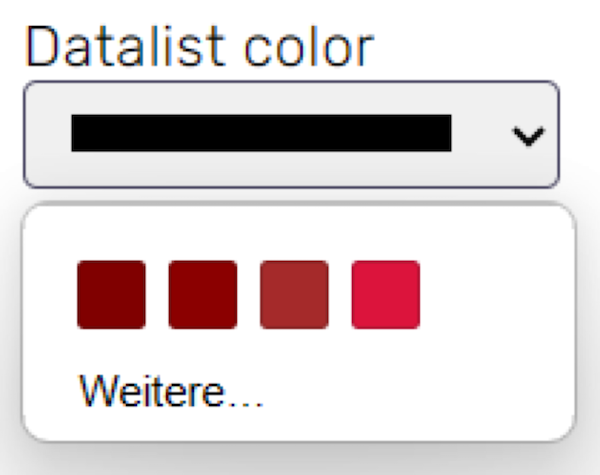
\includegraphics[width=0.9\textwidth]{color.win.edge.png}
        \caption{Color-Datalist auf Windows Edge}
        \label{img:colorWinEdgeDatalist}
    \end{minipage}
\end{figure}

% ---- specials - date --------

\begin{figure}[!htb]
    \centering
    \begin{minipage}[b]{0.28\textwidth}
        \centering
        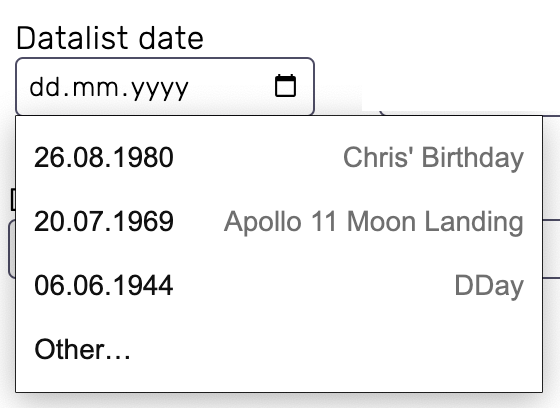
\includegraphics[width=0.9\textwidth]{date.osx.chrome.png}
        \caption{Date-Datalist auf OSX Chrome}
        \label{img:dateOsxChromeDatalist}
    \end{minipage}
    \hfill
    \begin{minipage}[b]{0.28\textwidth}
        \centering
        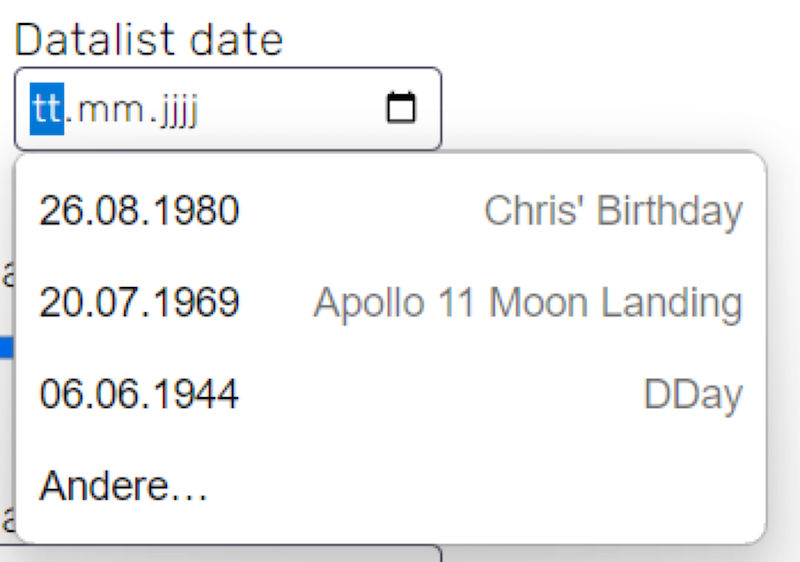
\includegraphics[width=0.9\textwidth]{date.win.chrome.png}
        \caption{Date-Datalist auf Windows Chrome}
        \label{img:dateWinChromeDatalist}
    \end{minipage}
    \hfill
    \begin{minipage}[b]{0.28\textwidth}
        \centering
        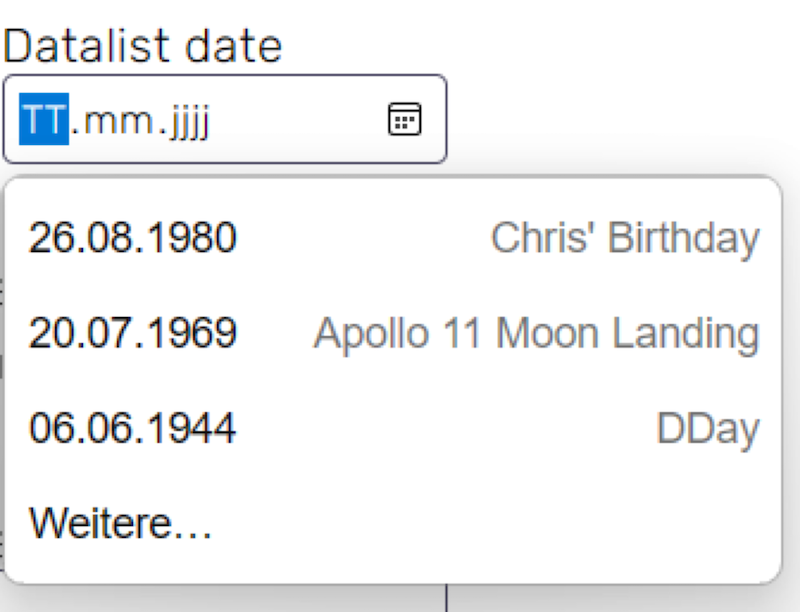
\includegraphics[width=0.9\textwidth]{date.win.edge.png}
        \caption{Date-Datalist auf Windows Edge}
        \label{img:dateWinEdgeDatalist}
    \end{minipage}
\end{figure}

% ---- specials - time --------

\begin{figure}[!htb]
    \centering
    \begin{minipage}[b]{0.28\textwidth}
        \centering
        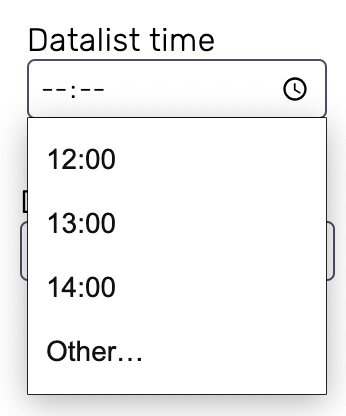
\includegraphics[width=0.9\textwidth]{time.osx.chrome.png}
        \caption{Time-Datalist auf OSX Chrome}
        \label{img:timeOsxChromeDatalist}
    \end{minipage}
    \hfill
    \begin{minipage}[b]{0.28\textwidth}
        \centering
        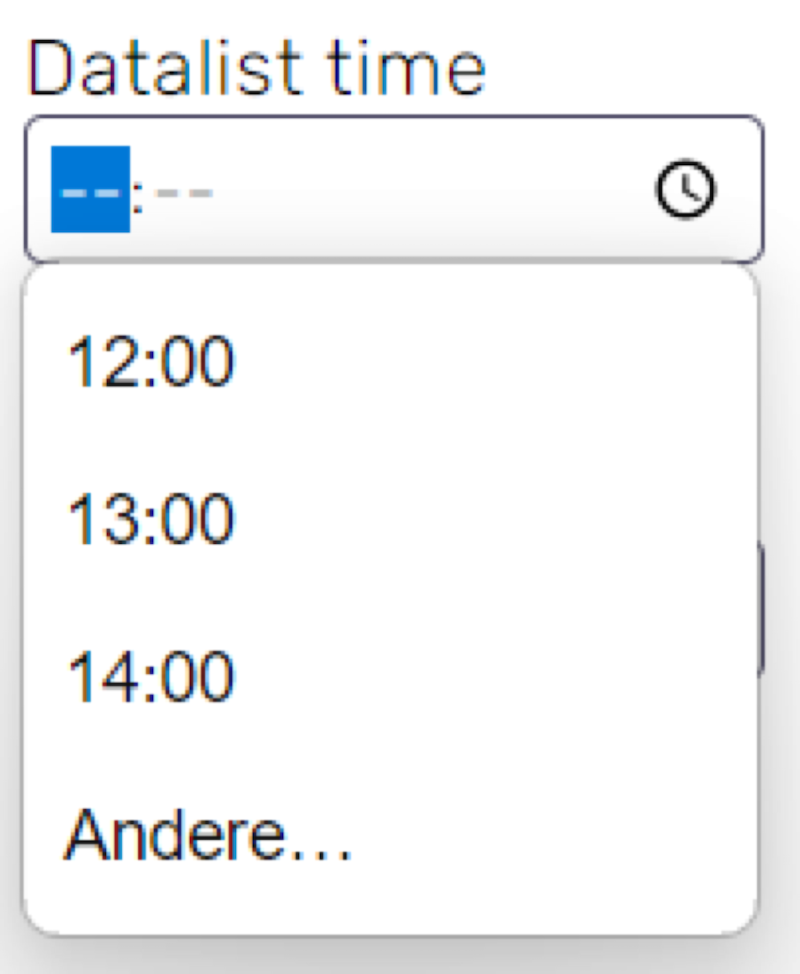
\includegraphics[width=0.9\textwidth]{time.win.chrome.png}
        \caption{Time-Datalist auf Windows Chrome}
        \label{img:timeWinChromeDatalist}
    \end{minipage}
    \hfill
    \begin{minipage}[b]{0.28\textwidth}
        \centering
        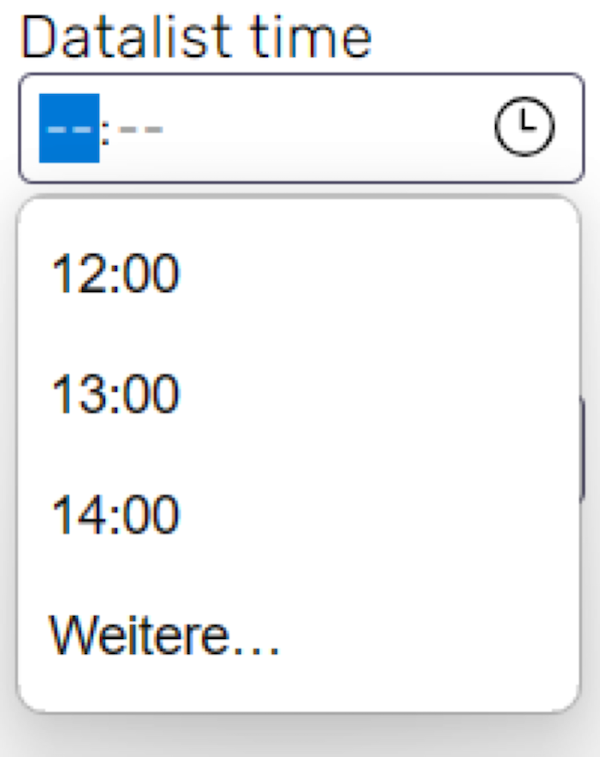
\includegraphics[width=0.9\textwidth]{time.win.edge.png}
        \caption{Time-Datalist auf Windows Edge}
        \label{img:timeWinEdgeDatalist}
    \end{minipage}
\end{figure}
